% !TeX root = ../main.tex
\chapter{相关理论基础}

\section{统计学习理论}

统计学习理论(Statistical Learning Theory,SLT)是Vapnik等人提出的一种专门研究小样本情况下机器学习问题的理论\cite{vapnik2013nature}。
SLT理论体系从已知数据出发,尝试学习数据背后所隐含的规律,并利用这些规则对未知数据进行分析。
该体系不仅考虑了对学习性能的要求,而且期望在有限的条件下得到最好的结果。
其核心包括:VC维,推广性的界和结构风险最小化原则。

\subsection{VC维}

VC维是SLT定义的一个评估学习机器的性能指标。

其定义为:对于假设函数空间$H$,如果存在大小为$n$的样本集合能够被函数空间$H$里的函数按所有可能的$2^n$方式分开,则称$H$能够将$n$个样本打散。
那么$H$所能打散的最大样本数目$n$为函数集的VC维,即:
\begin{align}
    \mathrm{VC}(H)=\mathrm{max}\{n:\Pi_H(n)=2^n\},
\end{align}
其中$\Pi_H(n)$为增长函数,即$H$能够将$n$个样本分开的最大结果数。

函数集的VC维代表了假设函数空间的复杂程度,VC维越大则假设函数空间越大,函数空间越复杂则学习机器的学习能力越强。

\subsection{推广性的界}

推广性(泛化误差)的界的研究内容为:各种类型函数集的实际风险(期望风险)和经验风险(训练误差)之间的关系。
对于二分类问题已有结论:对于假设空间中的所有函数,实际风险$R(\mathbf{w})$和经验风险$R(\mathbf{w})_{Empirical}$之间至少以概率$1-\eta$满足:
\begin{align}
    R(\mathbf{w})\leq R(\mathbf{w})_{Empirical} + \sqrt{\frac{h(\ln{\frac{2n}{h}+1}) - \ln{\frac{\eta}{4}}}{n}},
\end{align}
其中$h$为假设函数空间的VC维,$n$为样本数。

公式(2.2)说明了学习机器的实际风险$R(\mathbf{w})$是由两个部分组成的:经验风险(训练误差)和置信风险。
实际风险与样本的分布无关,只与学习机器的VC维和样本数量有关,能够简化为:
\begin{align}
    R(\mathbf{w})\leq R(\mathbf{w})_{Empirical} + \Phi(\frac{h}{n}).
\end{align}

公式(2.3)说明,在样本数量$n$确定的情况下,学习机器的VC维越高则置信风险越高,这将会导致过学习的现象。
学习机器不仅要使经验风险最小,还要使VC维尽量小来降低置信风险,从而使得学习机器对未知样本有良好的泛化能力。

\subsection{结构风险最小化原则}

以上说明,在小样本情况下,用经验风险来估计实际风险是不合理的。
为了解决这种问题,Vapnik提出了结构风险最小化原则,首先将函数集$S=\{f(\mathbf{x},a),a\in\Omega\}$分解为一个子序列$S_1, S_2, \ldots , S$,其中:
\begin{align}
    S_1\subset S_2\subset \ldots \subset S_k\subset \ldots \subset S,
\end{align}
使得每个子集能够按照VC维的大小排列,即:
\begin{align}
    h_1 < h_2 < \ldots h_k < \ldots < h.
\end{align}

SRM的基本思想是:在每个子集中寻找最小的经验风险,并在子集之间权衡经验风险和置信风险,使其总和实际风险达到最小。而支持向量机就是该思想的一种实现方式。

\section{支持向量机}

SVM是一种非概率性的监督学习模型,属于线性二元分类器其中最大间隔分类器中的一类。
因为SVM算法试图将高维数据映射到高维特征空间,并在此特征空间中构造一个能够满足要求的超平面,即在保证分类精度的同时,最大化超平面两侧的空白区域。
SVM专注于那些正好在最大间隔边缘上的训练向量,这些向量称之为支持向量。在训练阶段,只需考虑支持向量来决定训练向量的类。
由于支持向量的数量通常较少,所以该超平面分类精度最高,泛化能力最佳,此超平面被称为最大间隔超平面。

\begin{figure}[ht]
    \centering
    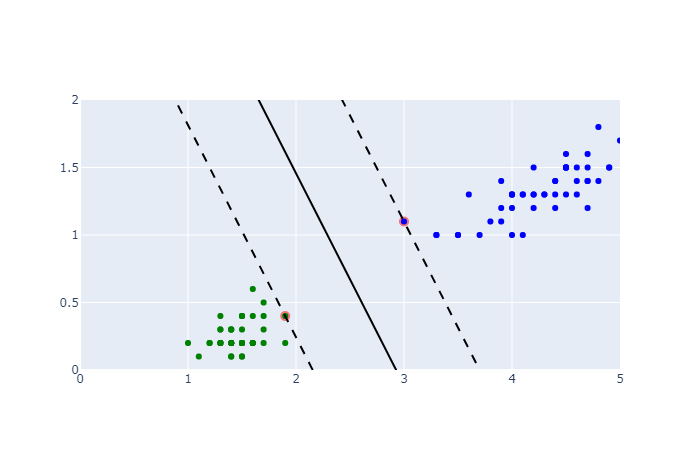
\includegraphics[scale=0.5]{1.png}
    \caption{最大间隔超平面}
\end{figure}

\subsection{最大间隔超平面}

考虑最简单的二分类问题,给定线性可分的训练样本$(\mathbf{x}_i,y_i),i=1,2,\ldots,n,(\mathbf{x}_i,y_i)\in\mathbb{R}^l\times\{-1,1\}$,
分割超平面由其权重向量$\mathbf{w}\in\mathbb{R}^n$和偏置$b\in\mathbb{R}$定义,其中偏置$b$定义了样本与超平面之间的距离。
于是,分割超平面可以被定义为决策函数:
\begin{align}
    f(\mathbf{x})=\mathbf{w}\cdot\mathbf{x}+b,
\end{align}
当$f(\mathbf{x})=0$时为超平面,为了使该超平面能够正确分类所有样本,就要求它满足如下约束:
\begin{align}
    y_i(\mathbf{w}\cdot\mathbf{x}_i+b)\geq1,\quad i=1,2,\ldots,n.
\end{align}
很容易得到分类间隔为$\frac{2}{\Vert\mathbf{w}\Vert}$,这个最大化问题能够非常方便地转化为等效的最小化$\frac{1}{2}\Vert\mathbf{w}\Vert^2$的问题。
因此,在样本空间中构造最优超平面的问题就被转化为在约束(2.7)下求解二次规划问题:
\begin{align}
    \min_{\mathbf{w},b}\frac{1}{2}\Vert\mathbf{w}\Vert^2.
\end{align}

为了解决这个约束最优化问题,我们引入Lagrange函数:
\begin{align}
    L(\mathbf{w},b,\alpha)=\frac{1}{2}\Vert\mathbf{w}\Vert^2+\sum_{i=1}^n\alpha_i[1-y_i(\mathbf{w}\cdot x_i+1)],
\end{align}
其中$\alpha_i\geq0, i=1,2,\ldots,n$为Lagrange乘数,通过对$\mathbf{w}$和$b$求一阶偏导并使之为0,我们得到对偶问题:
\begin{align}
    \min_\alpha\frac{1}{2}\sum_{i=1}^n\sum_{j=1}^ny_iy_j(\mathbf{x}_i\cdot\mathbf{x}_j)\alpha_i\alpha_j-\sum_{i=1}^n\alpha_i, \\
    s.t.\quad \sum_{i=1}^ny_i\alpha_i=0, \notag \\
    \alpha_i\geq0,i=1,2,\ldots,n.\notag
\end{align}
对于式(2.10),可以通过凸优化方法,例如序列最小优化算法(Sequential Minimal Optimization,SMO),
SMO算法将大的凸优化问题分解为一系列小的等效凸优化问题,并一个个解决它们。
由此求出最优解$\alpha^*=(\alpha_1^*,\alpha_2^*,\ldots,\alpha_n^*)^\mathrm{T}$,
然后计算最优权重向量$\mathbf{w}^*$和最优偏置$b^*$,即:
\begin{align}
    \mathbf{w}^*=\sum_{i=1}^n\alpha_i^*y_i\mathbf{x}_i, \\
    b^*=y_i-\sum_{j=1}^ny_j(\mathbf{x}_j\cdot\mathbf{x}_i)\alpha_j^*.
\end{align}
其中$j\in\{j|\alpha_j^*>0\}$,这些点位于最大间隔的边界上,说明定义决策函数的权重向量$\mathbf{w}$与偏置$b$。
最后,决策函数可以表示为:
\begin{align}
    f(\mathbf{x})=\mathrm{sign}(\sum_{i=1}^n\alpha_i^*y_i\mathbf{x_i}\cdot\mathbf{x}+b).
\end{align}
从中我们可以看到,支持向量机对内存的消耗是巨大的,大量的计算资源将被用在点乘的计算上。

\subsection{软间隔超平面}

线性SVM有一个局限:如果样本数据不是线性可分的,那么就无法找到以上的超平面。
针对此类问题,软间隔支持向量机实现了一个新的成本函数,引入了松弛变量(Slack variables)$\xi$,来作为惩罚被错误分类样本数据的损失项:
\begin{align}
    \min_{\mathbf{w},b}\frac{1}{2}\Vert\mathbf{w}\Vert^2+C\sum_{i=1}^n\xi_i,\\
    s.t.\quad y_i(\mathbf{w}\cdot\mathbf{x}_i+b)-1+\xi_i\geq0,\notag\\
    \xi_i\geq0,i=1,2,\ldots,n.\notag
\end{align}
其中,$\sum_{i=1}^n\xi_i$可以看成错误分类样本数量的某种度量。
同时,引入一个正则化常数$C\in[0,\infty)$来控制最小化$\frac{1}{2}\Vert\mathbf{w}\Vert^2$的权重,并且对具有非常大$\xi_i$的解进行惩罚。
事实上,$C$可以被认为是权衡模型泛化能力和训练误差的参数,这取决于它的值。

\begin{figure}[ht]
    \centering
    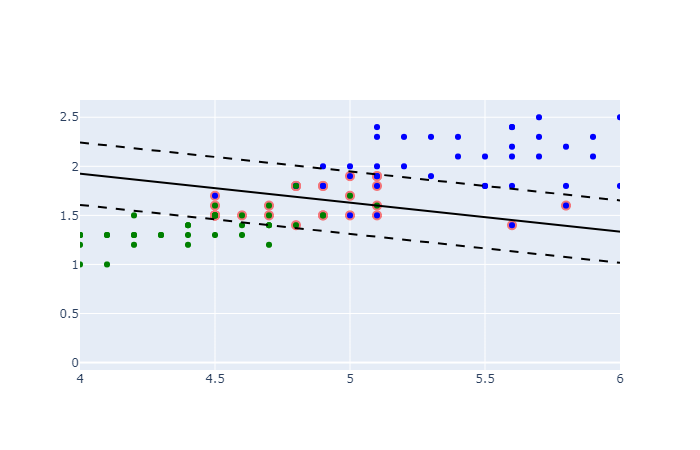
\includegraphics[scale=0.5]{2.png}
    \caption{软间隔超平面}
\end{figure}

再一次,我们一样可以利用Lagrange函数来将原始问题转化为凸优化问题,只需引入约束$C\geq\alpha_i\geq0$,因为松弛变量$\xi_i$对优化问题没有任何影响。

\subsection{核函数}

作为软间隔超平面实现的替代方案,SVM方法可以通过在分类器中加入一个内核来进行非线性分类。
其主要思想是将原始特征向量$x_i\in\mathbb{R}^n$通过一个非线性向量函数$\Phi: \mathbb{R}^n\to\mathcal{H}$映射到一个更高维的欧几里得空间,即$\mathcal{H}$。
在此高维特征空间中,将变换后的向量$\Phi(\mathbf{x_i})\cdot\Phi(\mathbf{x})$代替样本的原始内积$\mathbf{x}_i\cdot\mathbf{x}$,得到决策函数:
\begin{align}
    f(\mathbf{x})=\mathrm{sign}(\sum_{i=1}^n\alpha_i^*y_iK(\mathbf{x}_i,\mathbf{x})+b),
\end{align}
其中$K(\mathbf{x}_i,\mathbf{x})=\Phi(\mathbf{x_i})\cdot\Phi(\mathbf{x})$。

方程(2.14)的假设可以避免计算转换后向量之间的内积,大大减少了算法的计算消耗。另外,为了确保底层映射$\Phi$的存在,内核函数必须满足Mercer条件\cite{en1}。

最后,对偶问题被表示为:
\begin{align}
    \min_\alpha\frac{1}{2}\sum_{i=1}^n\sum_{j=1}^ny_iy_jK(\mathbf{x}_i,\mathbf{x}_j)\alpha_i\alpha_j-\sum_{i=1}^n\alpha_i, \\
    s.t.\quad \sum_{i=1}^ny_i\alpha_i=0, \notag \\
    C\geq\alpha_i\geq0,i=1,2,\ldots,n.\notag
\end{align}

\begin{table}[ht]
    \centering
    \caption{SVM常用核函数,其中$\gamma$为超参数,$d$为阶数}
    \begin{tabular}{lc}
        \hline
        {名称} & {函数形式}\\
        \hline
        {线性核函数} & {$\mathbf{x}_i\cdot\mathbf{x}_j$}\\
        {多项式核函数} & {$(\gamma\mathbf{x}_i\cdot\mathbf{x}_j+1)^d$}\\
        {Sigmoid核函数} & {$\mathrm{tanh}(\gamma\mathbf{x}_i\cdot\mathbf{x}_j+c)$}\\
        {径向基核函数(Radical Basis Function,RBF)} & {$\mathrm{exp}(-\gamma\Vert\mathbf{x}_i-\mathbf{x}_j\Vert^2)$}\\
        \hline
    \end{tabular}
\end{table}

内核函数隐式地定义了特征空间,因此内核函数的选择对SVM的性能至关重要,如果样本被映射到一个不合适的特征空间,将导致SVM的泛化能力降低。
事实上,内核函数通常测量输入样本$\mathbf{x}_i$和其他训练样本$\mathbf{x}_j$之间的距离,表(2.1)展示了一些常用的内核函数。
特别是RBF内核$\mathrm{exp}(-\gamma\Vert\mathbf{x}_i-\mathbf{x}_j\Vert^2)$,它具有相当有趣的特性:
其中$\gamma$控制着模型的性能,从这个意义上来说,低的$\gamma$值会提供低偏差高方差的分类结果,而高的$\gamma$值会提供高偏差和低方差的结果。

其中,线性核函数适用于线性可分的情况,但现实世界多为非线性问题,较少使用;多项式核函数在全局上表现良好,但参数较多,训练速度较慢;
Sigmoid几乎不使用,在一些条件下甚至是无法使用的;径向基函数性能比较稳定,是目前应用最广的核函数。